\documentclass{article}
\linespread{1.3}
\usepackage[margin=50pt]{geometry}
\usepackage{amsmath, amsthm, amssymb, amsthm,fancyhdr, graphicx, tikz}
\pagestyle{fancy}
\renewcommand{\headrulewidth}{0pt}
\newcommand{\changefont}{\fontsize{15}{15}\selectfont}

\fancypagestyle{firstpageheader}
{
  \fancyhead[R]{\changefont Michael Huang \\ Homework 6 \\ Adekoya}
}

\begin{document}

\thispagestyle{firstpageheader}

\section*{2.}
{\Large
The random variable $X$ has the following probability density function:
\[
f\left(t\right)=\begin{cases}
ct^{2} & \,-1\le t\le,2;\\
0 & \,\mbox{otherwise,}
\end{cases}
\]
where $c$ is a constant.

\subsection*{(a)}
To find $c$, we aim to solve for $c$ in the equation $\int_{-1}^{2}  ct^2\,dx = 1$, since we know that the total probability must be 1. Solving this: \\ 
$\frac{ct^3}{3}|_{-1}^{2} = 1$ \\ 
$\frac{8c}{3} + \frac{c}{3} = 1$ \\ 
$3c = 1$ \\ 
\framebox[1.1\width]{\textbf{c = $\frac{1}{3}$}}

\begin{figure}[ht!]
  \centering
  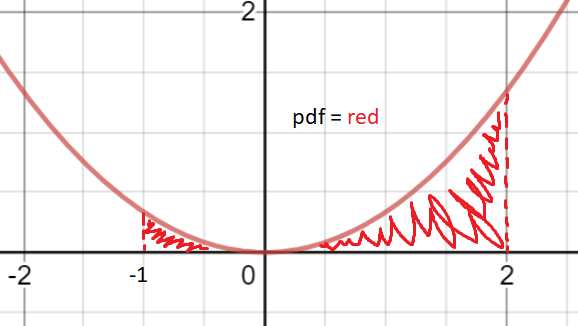
\includegraphics[width=90mm]{pdf.PNG}
  \caption{pdf \label{overflow}}
\end{figure}

\begin{figure}[ht!]
  \centering
  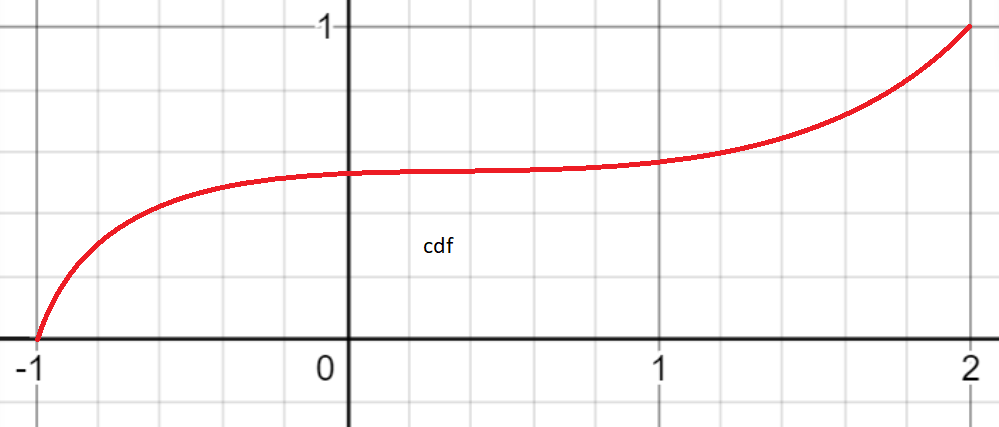
\includegraphics[width=90mm]{cdf.PNG}
  \caption{cdf; note EXTREMELY NOT TO SCALE \label{overflow}}
\end{figure}

\subsection*{(b)}
By definition, E($X$) = $\int_{-\infty}^{\infty}x \cdot f(x) \,dx$. Solving this, we get E($X$)  \\ 
$ = \int_{-1}^{2} \frac{x^3}{3} \,dx$ \\ 
$ = \frac{x^4}{12} |_{-1}^{2}$ \\ 
$ = \frac{2^4}{12} - \frac{-1^4}{12}$ \\ 
$ = \frac{15}{12}$ \\
= \framebox[1.1\width]{\textbf{$\frac{5}{4}$}} \\ \\
By definition, $Var(X$) = E($X^2$) - E$(X)^2$. We have E($X$) already, so we find E($X^2$): \\ 
E($X^2$) = $ \int_{-1}^{2} x^2 \cdot \frac{x^2}{3} \,dx$ \\ 
$ = \int_{-1}^{2} \frac{x^4}{3} \,dx$ \\
$ = \frac{x^5}{15} |_{-1}^{2}$ \\
$ = \frac{2^5}{15} - \frac{-1^5}{15}$ \\
$ = \frac{33}{15}$ \\ \\ 
We can thus find $Var(X$) = E($X^2$) - E$(X)^2$ = $\frac{33}{15} - \frac{25}{16} = $ \framebox[1.1\width]{\textbf{$\frac{51}{80}$}} 

\subsection*{(c)}
The CDF of Y $F_Y(y) = P(Y \leq y) = P(X^2 \leq y) = P(X \leq \sqrt{y}) = F_X(\sqrt{y})$. \\
To find the density function $f_Y$, we need to find the derivative of $F_Y(y) = \frac{d}{dy}F_Y(y) = \frac{d}{dy}(F_X(\sqrt{y})) = {F'}_X(\sqrt{y}) \cdot \frac{1}{2\sqrt{y}} = \frac{1}{2\sqrt{y}}f_X(\sqrt{y}) = \frac{}{}$
\[
\begin{cases}
\frac{t^2}{3} & \,-1\le t\le,2;\\
0 & \,\mbox{otherwise,}
\end{cases}
\]

\subsection*{(d)}
Find E($X^2$) using the density $f_Y(t)$

}

\section*{3.}
{\Large 
Let $X$ be a random variable with the following density function
\[
f_{X}\left(t\right)=\begin{cases}
bt+b & \,-1<t<0;\\
-\frac{bt}{3}+b & \,0\le t<3\\
0 & \,\mbox{otherwise.}
\end{cases}
\]

\subsection*{(a)}
To find $b$, we need to find each respective CDF and add them to 1, since by definition we have a total probability of 1. Solving this: \\ 
$1 = \int_{-1}^{0} bt + b \,dt + \int_{0}^{3} -\frac{bt}{3} + b \,dt$ \\ 
$1 =  (\frac{bt^2}{2} + bt) |_{-1}^{0} + (-\frac{bt^2}{6} + bt) |_{0}^{3}$ \\ 
$1 =  -\frac{b}{2} + b + -\frac{9b}{6} + 3b$ \\ 
$1 =  2b$ \\ 
\framebox[1.1\width]{\textbf{$b = \frac{1}{2}$}}

\subsection*{(b)}
By definition, the cdf $F_X(a) = \int_{-\infty}^{a} f(x) \,dx$, so we take the integrals of functions and compound them onto each other. \\
First, we know that for any $t < -1$, the cdf is simply 0, since our pdf is simply 0 there. \\
Next, for the range $\{-1, 0\}$ we have $\int_{-\infty}^{-1} 0 \,dt + \int_{-1}^{t} \frac{t}{2} + \frac{1}{2} \,dt$ \\
$ = 0 + (\frac{t^2}{4} + \frac{t}{2}) |_{-1}^{t}$ \\ 
$ = \frac{t^2}{4} + \frac{t}{2} - (\frac{1}{4} + \frac{-1}{2})$ \\
$ = \frac{t^2}{4} + \frac{t}{2} + \frac{1}{4}$ \\ 
Finally, for the range $[0, 3\}$, we have $\int_{-\infty}^{-1} 0 \,dt + \int_{-1}^{0} \frac{t}{2}+ \frac{1}{2} \,dt + \int_{0}^{t} -\frac{t}{6} + \frac{1}{2} \,dt$ \\
$= 0 + (\frac{t^2}{4} + \frac{t}{2}) |_{-1}^{0} + (-\frac{t^2}{12} + \frac{t}{2}) |_{0}^{t}$ \\
$= -(\frac{1}{4} + \frac{-1}{2}) + -\frac{t^2}{12} + \frac{t}{2}$ \\
$=  -\frac{t^2}{12} + \frac{t}{2} + \frac{1}{4}$ \\
We also know by definition that for any greater value, the cdf will simply be 1. \\
Therefore, our cdf is 
\[
F_{X}\left(t\right)=\begin{cases}
0 & \,t<-1;\\
\frac{t^2}{4} + \frac{t}{2} + \frac{1}{4} & \,-1<t<0;\\
-\frac{t^2}{3} + \frac{t}{2} + \frac{1}{4} & \,0 \leq t < 3;\\
1 & \,t\geq 3;\\
\end{cases}
\]

\subsection*{(c)}


\subsection*{(d)}


}

\section*{4.}
{\Large 
Two young squirrels are playing tug of war with a twig. Suppose that the twig breaks at a location that is equally likely to be at any point along the length of the twig. One of the squirrels will cry if its piece of the twig is less than half the size of the other squirrel's piece of the twig. What is the probability that one of the squirrels ends up crying? \\ \\
If we consider that the entire probability space of where the twig breaks to total 1, we can consider that the first squirrel will cry if location $x$ on the twig is such that $x \leq \frac{1 - x}{2}$, and the second squirrel will cry in the same situation if $(1 - x) \leq \frac{x}{2}$. Isolating $x$ in both equations, we can find that $3x \leq 1$ and $2 \leq 3x$. Equivalently, we have the inequalities $x \leq \frac{1}{3}$ and $\frac{2}{3} \leq x$ that represent when the squirrel will cry. We can therefore see that if $x$ is in the lowest third or highest third, a squirrel will cry, for a total of $\frac{1}{3} + \frac{1}{3} =$ \framebox[1.1\width]{\textbf{$\frac{2}{3}$}}  probability that a squirrel will cry.

}

\section*{5.}
{\Large 
The rainfall can be modeled with $X \sim N(40, 16)$, $P(X > 50) = 1 - P(X \leq 50) = 1 - \Phi(\frac{50 - 40}{4}) = 1 - \Phi(\frac{5}{2}) = 0.0062$, which we used the normal distribution table to calculate. If we assume that annual rainfall is independent every year, we can then just model this by taking the probability that we won't get rainfall above 50 inches for 10 years, which is simply just \\ \\ 
$(1 - 0.0062)^{10} = 0.9938^{10} = $ \framebox[1.1\width]{\textbf{0.93970150864}}

}

\section*{6.}
{\Large 
Suppose that X is a normal r.v. with mean 5. If P($X > 9$) = 0.2, then find $Var(X)$. \\ 
We can model $X \sim N(5, \sigma^2)$. We know that $P(X > 9) = 0.2$, which also means that $P(X \leq 9) = 1 - 0.2 = 0.8$. By definition, $P(X \leq 9)$ = $\Phi(\frac{9 - 5}{\sigma}) = \Phi(\frac{4}{\sigma}) = 0.8$. Referencing the normal distribution table to determine $\frac{4}{\sigma} = \Phi^{-1}(0.8) = $ $\sim0.845$. Therefore, we can solve for $\sigma = \frac{4}{0.845} = 4.73372781065$. We know that $Var(X) = \sigma^2 = $ \framebox[1.1\width]{\textbf{22.4081789853}}

}

\section*{7.}
{\Large 
Suppose $X\sim\mathrm N({0,1})$, and let $Y=X^{2}$. Find the cdf and pdf of $Y$ in terms of $\phi$ (the cdf of $X$). \\
To find the cdf of Y $F_y$: \\
$= P(Y \leq y) = P(X^2 \leq y)$ \\ 
$= P(-\sqrt{y} \leq X \leq \sqrt{y})$ \\
$ = \Phi(\sqrt{y}) - \Phi(-\sqrt{y})$ \\
$ = \Phi(\sqrt{y}) - (1 - \Phi(\sqrt{y}))$ \\
= \framebox[1.1\width]{\textbf{$2\Phi(\sqrt{y}) - 1$}} \\ 
To find the pdf, we simply take the derivative: \\ 
$ = \frac{d}{dy} (2\Phi(\sqrt{y}) - 1)$ \\ 
$ = 2\Phi'(\sqrt{y}) \cdot \frac{1}{2\sqrt{y}}$ \\ 
= \framebox[1.1\width]{\textbf{$\Phi'(\sqrt{y}) \cdot \frac{1}{\sqrt{y}}$}}

}

\section*{8.}
{\Large 

\subsection*{(a)}
We can model this using a Binomial random variable. We know that we multiply by 1.0005 if the stock rises (consider this a "win"), and by 0.9995 if the stock decreases (consider this a "loss"). The price changes every second, so within an hour, we have 60 * 60 = 3600 rounds. Therefore, we can solve to find the point at which the price will end at 105 or 1.05 times the original price, that is how many "wins" or increases versus "losses" or decreases are necessary to get to an ending price of 105. To calculate this, we take \\ 
$1.05 \leq 1.0005^{k} \cdot 0.9995^{3600 - k}$ \\ 
$\ln(1.05) \leq \ln(1.0005^{k} \cdot 0.9995^{3600 - k})$ \\ 
$\ln(1.05) \leq \ln(1.0005^{k}) + \ln(0.9995^{3600 - k})$ \\ 
$\ln(1.05) \leq k \cdot \ln(1.0005) + (3600 - k) \cdot \ln(0.9995)$ \\ 
$\ln(1.05) \leq k \cdot \ln(1.0005) + 3600 \cdot \ln(0.9995) - k \cdot \ln(0.9995)$ \\ 
$\ln(1.05) - 3600 \cdot \ln(0.9995) \leq k \cdot \ln(1.0005) - k \cdot \ln(0.9995)$ \\ 
$k \geq \frac{\ln(1.05) - 3600\ln(0.9995)}{\ln(1.0005) - \ln(0.9995)}$ \\
$k \geq 1849.24016012$ \\ 
Since we cannot make fractional trades, we need at least 1850 "wins" or increases to end the hour at 105. At this point, we can use the fact that the binomial random variable is derived from the normal distribution. By definition, we know that for $X \sim $ Bin($3600, 0.51$), E($X$) = $np = 3600 \cdot 0.51 = 1836$, while $Var(X) = np(1 - p) = 3600 \cdot 0.51 \cdot (1 - 0.51) = 899.64$, and therefore $\sigma = \sqrt{Var(X)} = \sim 29.994$. We therefore can define the distribution as $X \sim N(1836, 29.994)$, and can subsequently find that $P(X \geq 1850) = 1 - \Phi(\frac{1850 - 1836}{29.994}) = 1 - \Phi(\frac{14}{29.994}) = 1 - \sim 0.68082 = $ \framebox[1.1\width]{\textbf{$\sim$ 0.31918}}

\subsection*{(b)}
We can model this using a Binomial random variable. We know that we multiply by 1.0005 if the stock rises (consider this a "win"), and by 0.9995 if the stock decreases (consider this a "loss"). The price changes every second, so within an hour, we have 60 * 60 = 3600 rounds. Therefore, we can solve to find the point at which the price will end at 105 or 1.05 times the original price, that is how many "wins" or increases versus "losses" or decreases are necessary to get to an ending price of 105. To calculate this, we take \\ 
$1.05 \leq 1.0005^{k} \cdot 0.9995^{3600 - k}$ \\ 
$\ln(1.05) \leq \ln(1.0005^{k} \cdot 0.9995^{3600 - k})$ \\ 
$\ln(1.05) \leq \ln(1.0005^{k}) + \ln(0.9995^{3600 - k})$ \\ 
$\ln(1.05) \leq k \cdot \ln(1.0005) + (3600 - k) \cdot \ln(0.9995)$ \\ 
$\ln(1.05) \leq k \cdot \ln(1.0005) + 3600 \cdot \ln(0.9995) - k \cdot \ln(0.9995)$ \\ 
$\ln(1.05) - 3600 \cdot \ln(0.9995) \leq k \cdot \ln(1.0005) - k \cdot \ln(0.9995)$ \\ 
$k \geq \frac{\ln(1.05) - 3600\ln(0.9995)}{\ln(1.0005) - \ln(0.9995)}$ \\
$k \geq 1849.24016012$ \\ 
Since we cannot make fractional trades, we need at least 1850 "wins" or increases to end the hour at 105. At this point, we can use the fact that the binomial random variable is derived from the normal distribution. By definition, we know that for $X \sim $ Bin($3600, 0.51$), E($X$) = $np = 3600 \cdot 0.5 = 1800$, while $Var(X) = np(1 - p) = 3600 \cdot 0.5 \cdot (1 - 0.5) = 900$, and therefore $\sigma = \sqrt{Var(X)} = 30$. We therefore can define the distribution as $X \sim N(1800, 30)$, and can subsequently find that $P(X \geq 1850) = 1 - \Phi(\frac{1850 - 1800}{30}) = 1 - \Phi(\frac{50}{30}) = 1 - \sim 0.94520 = $ \framebox[1.1\width]{\textbf{$\sim$ 0.05480}} \\ \\ 
I don't think that this is a realistic model since the randomness is modeled to be very independent and not compound upon each other (e.g. no trends in dips/rallies are taken into account). Trader sentiment is very real, which can often make the fluctuation of price in real time much more momentous than random or independent.

}

\section*{9.}
{\Large 
Suppose $X,Y$ are continuous random variables, with cumulative distribution
functions (cdfs) $F_{X}$ and $F_{Y}$, respectively. For each of
the following, determine whether the function $F$ is necessarily
the cdf of some random variable $Z$? In case the function is a cdf,
find the density $f_{Z}$ in terms of $F_{X}$, $f_{X}$, $F_{Y}$
and $f_{Y}$. If the function is not necessarily a cdf, give an example
of random variables $X,Y$ such that the function is not a cdf. 

\subsection*{(a)}
$F\left(t\right)=\frac{F_{X}\left(t\right)+2F_{Y}\left(t\right)}{3}$.

\subsection*{(b)}
$F\left(t\right)=F_{X}\left(t\right)\cdot F_{Y}\left(t\right)$.

\subsection*{(c)}
$F\left(t\right)=F_{X}\left(F_{Y}\left(t\right)\right)$.


}

\end{document}